\documentclass[border=2pt]{standalone}

%Drawing
\usepackage{tikz}
\tikzset{>=latex}
\usetikzlibrary{calc, decorations.markings}

%Styles
%%Arrow in the Middle
\tikzset{arrow inside/.style = {postaction=decorate,decoration={markings,mark=at position 0.52 with \arrow{stealth}}}}

% Colors
\definecolor{glass}{cmyk}{0.2,0,0,0}

% Newcommand
%% Mid Line Label
\newcommand{\midlabelline}[3]{
   \node (midlabel) at ($ (#1)!.5!(#2) $) {#3};
   \draw[<-] (#1) --  (midlabel);
   \draw[->] (midlabel) -- (#2);
}

\begin{document}
	
	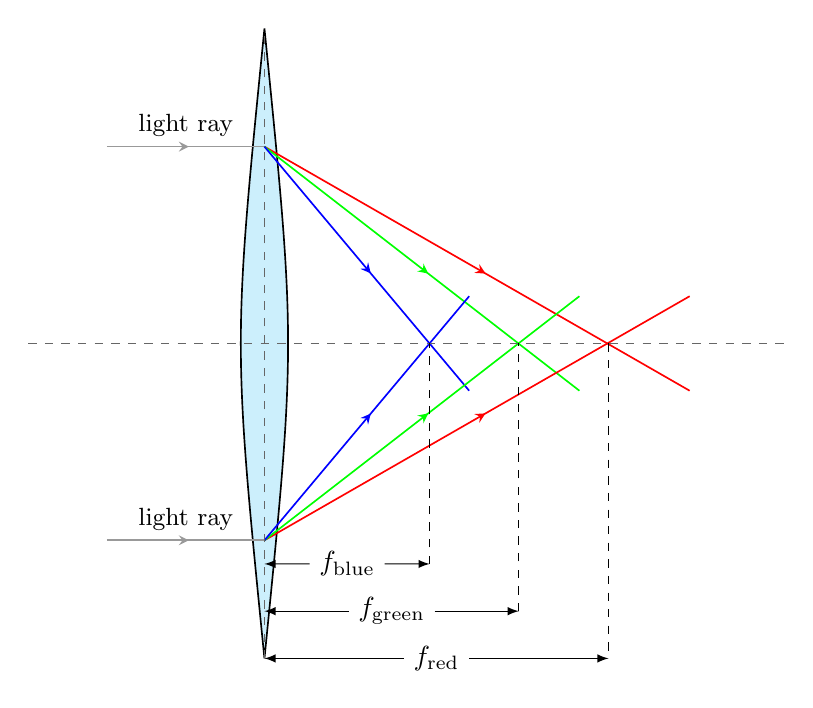
\begin{tikzpicture}[scale=2]
		% Grid
%		\draw[help lines] (-1,-2) grid (4,2);
%		\foreach \i in {0,0.5,1,1.5,...,5}
%		{
%			\node at (\i,-2ex) {$\i$};
%		}
		
		% Lens
		\path[fill=glass, draw=black, line width = 0.6] (1,-2) .. controls (0.8,0) .. (1,2) .. controls (1.2,0) .. (1,-2);
		
		% Rays
		\draw[black!40, line width = 0.6, arrow inside] (0,1.25) -- (1,1.25) node[above, pos=0.5, black] {\small light ray};
		%
		\draw[red, line width = 0.6, arrow inside] (1,1.25) -- (3.7,-0.3);	
		\draw[green, line width = 0.6, arrow inside] (1,1.25) -- (3,-0.3);	
		\draw[blue, line width = 0.6, arrow inside] (1,1.25) -- (2.3,-0.3);	
		%
		\draw[black!40, line width = 0.6, arrow inside] (0,-1.25) -- (1,-1.25) node[above, pos=0.5, black] {\small light ray};
		%
		\draw[red, line width = 0.6, arrow inside] (1,-1.25) -- (3.7,0.3);	
		\draw[green, line width = 0.6, arrow inside] (1,-1.25) -- (3,0.3);	
		\draw[blue, line width = 0.6, arrow inside] (1,-1.25) -- (2.3,+0.3);	
		
		% Axis
		\draw[dashed, black!60] (1,-2) -- +(0,4);
		\draw[dashed, black!60] (-0.5,0) -- (4.3,0);
		
		% Focal Points
		\midlabelline{1,-1.7}{2.615,-1.7}{$f_\mathrm{green}$}
		\draw[dashed] (2.615,-1.7) -- (2.615,0);
		%
		\midlabelline{1,-2}{3.185,-2}{$f_\mathrm{red}$}
		\draw[dashed] (3.185,0) -- (3.185,-2);
		%
		\midlabelline{1,-1.4}{2.049,-1.4}{$f_\mathrm{blue}$}
		\draw[dashed] (2.049,-1.4) -- (2.049,0);
	\end{tikzpicture}
	
\end{document}
